%%% Class Diagram subsection
%%% Version 2
% Class diagrams are the most common diagram type in object-oriented modeling. 
% They illustrate the static structure of a system by depicting classes, their 
% attributes, operations, and the relationships between classes. Classes 
% represent sets of objects, where attributes describe the values these objects 
% may contain, and operations specify the behaviors objects can perform.
% Associations in class diagrams describe connections between different classes, 
% with multiplicity indicators showing how many objects of one class can be linked 
% to objects of another class. Class diagrams also include other relationship types: 
% aggregation and composition (both representing whole-part relationships, with 
% different levels of dependency), and generalization (inheritance relationship 
% where specialized classes inherit properties from a general class).

% % Example here
% \begin{figure}
%     \begin{center}
%         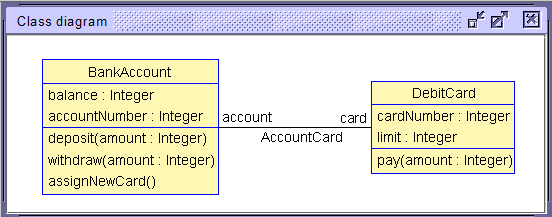
\includegraphics[width=0.8\textwidth]{figures/c1/BankAccount/BankAccount_ClassDiagram.png}
%         \caption{Class diagram of the Bank Account Model.}
%         \label{fig:class_diagram_bank_account_model}
%     \end{center}
% \end{figure}

% Figure \ref{fig:class_diagram_bank_account_model} shows an example class diagram
% of a bank account system. The system can have multiple bank accounts and each account 
% can have multiple debit cards. The class diagram consists of the classes BankAccount 
% and DebitCard with the association AccountCard. The class BankAccount has two attributes:
% - accountNumber: a unique identifier for the bank account.
% - balance: the current balance of the bank account.
% and the class DebitCard has two attributes:
% - cardNumber: a unique identifier for the debit card.
% - limit: the maximum amount that can be withdrawn using the debit card.

% The class diagram can also have other elements such as aggregation, composition
%  and generalization to show the relationship between classes. Aggregation and compo
% sition are a whole-part relationship. In aggregation, the relationship between a child
%  class and parent class is independent, whereas, in composition, they are dependent.
%  A generalization is a relationship between classes in which one class is identified as
%  the general class and the others as the specialization of it. A specialized class inherits
%  all the properties and characteristics from the general class.

%%% Version 1
% Class diagrams show the static structure of a system by depicting classes, 
% their attributes, operations, and relationships between classes. These diagrams 
% form the foundation of object-oriented modeling and capture how objects relate 
% to one another. Class diagrams are important for understanding the system structure 
% that our temporal and event-based extensions will work with.

%%% Sample
% Class diagrams are the most common diagram found in object-oriented modeling
%  systems. It illustrates the static design view of the system model and shows classes
%  of the system, their attributes, operations and associations [64]. The classes reflect
%  a set of objects. The attributes describe values that the objects may contain, and
%  an operation specifies the result of the behavior of objects. The associations describe
%  connections among the different class objects, and they can refer to each other through
%  role names. The number of objects of one class linked to other class objects depends
%  on the multiplicity attached to an association end.
% The class diagram can also have other elements such as aggregation, composition
% and generalization to show the relationship between classes. Aggregation and compo
% sition are a whole-part relationship. In aggregation, the relationship between a child
% class and parent class is independent, whereas, in composition, they are dependent.
% A generalization is a relationship between classes in which one class is identified as
% the general class and the others as the specialization of it. A specialized class inherits
% all the properties and characteristics from the general class.

%%% Object Diagram subsection
%%% Version 1
% Object diagrams provide snapshots of a system at specific points in time, showing 
% actual instances of classes (objects) and their relationships. While class diagrams 
% show abstract structures, object diagrams show concrete system states with specific 
% values. These diagrams are useful for verification purposes as they show examples 
% of system configurations that meet or violate constraints. In this thesis, object 
% diagrams play an important role in validating temporal properties through the 
% filmstrip approach.

%%% Sample
% Object diagrams are also a type of structural diagram. It represents the entitites of the
%  real world, or of the modeled system, as instances of the classes described in the class
%  diagram, and their relationships as links, which are instances of the corresponding
%  associations. Objects are defined by concrete attribute values and a link connects
%  the objects participating in the association. In general, an object diagram provides
%  a snapshot of a system at a particular point in time showing objects, their attribute
%  values, and links connecting the objects [77].
% The object diagram represents only the single state of a class diagram. So, the
%  previous state information can be lost due to the change in the system state through
%  the operation call. Therefore, a single object diagram cannot represent any flow of
%  information of a state.